%%%%%%%%%%%%%%%%%%%%%%%%%%%%%%%%%%%%%%%%%%%%%%%%%
%%                                             %%
%%               PhD Thesis                    %%
%%                                             %%
%%%%%%%%%%%%%%%%%%%%%%%%%%%%%%%%%%%%%%%%%%%%%%%%%

%% Authors: Séverin Lemaignan


\documentclass[a4paper,12pt]{book}

\usepackage{fullpage}

\usepackage{graphicx}

\usepackage{xcolor}

\usepackage{ifthen}

\usepackage[utf8]{inputenc}

\usepackage[T1]{fontenc}
\pdfmapfile{+ubuntu-regular.map}
\pdfmapfile{+ubuntu-it.map}
\pdfmapfile{+ubuntu-bold.map}
\renewcommand{\rmdefault}{Ubuntu}

\usepackage{listings}
\usepackage{alltt}
\usepackage{pseudocode}
\usepackage{framed}
\usepackage{wrapfig}
\usepackage{fancyhdr} %headers and footers
\pagestyle{fancy}

\usepackage{url}
\usepackage{hyperref}
\usepackage{sectsty}

\usepackage{enumerate}
\usepackage{paralist}

\usepackage{pdfpages} %% To add a cover to the doc

% Fixme notes
\usepackage[draft,footnote,marginclue]{fixme}

\usepackage[toc]{glossaries}

\usepackage[english]{babel}

%%%%%%%%%%%%%%%%%%%%%%%%%%%%%%%%%%%%%%%%%%%%%%%%%%%%%%%%%%%%%%%%%%%%%%%%%%%%%%%
%%                           Glossary                                        %%
%%%%%%%%%%%%%%%%%%%%%%%%%%%%%%%%%%%%%%%%%%%%%%%%%%%%%%%%%%%%%%%%%%%%%%%%%%%%%%%
\makeglossaries
%Pour re-générer le glossaire : makeindex squeakbot_pas_a_pas.glo -s squeakbot_pas_a_pas.ist -t squeakbot_pas_a_pas.glg -o squeakbot_pas_a_pas.gls
%\newglossaryentry{parametre}
%		{name={paramètre}, 
%		description={Un paramètre d'une fonction est une option que l'on passe à la fonction et que l'on peut modifier.}}
%%%%%%%%%%%%%%%%%%%%%%%%%%%%%%%%%%%%%%%%%%%%%%%%%%%%%%%%%%%%%%%%%%%%%%%%%%%%%%%

%Name of the speaker in a chat
\newcommand{\chatN}[1]{{\footnotesize \textsf{#1}}}
\newcommand{\concept}[1]{{\footnotesize \texttt{#1}}}

\newcommand{\stmt}[1]{{\footnotesize \tt $\langle$ #1\relax$\rangle$}}
%\newcommand{\stmt}[1]{{\footnotesize $\langle$\stmttt#1\relax$\rangle$}}
\newcommand{\rawstmt}[1]{{\footnotesize \stmttt#1\relax}}
\def\stmttt#1 #2 #3\relax{{\tt#1} {\bf{\tt #2}} {\tt #3}}

\newcommand{\setstmt}[1]{{\footnotesize [\setstmttt#1\relax]}}
\def\setstmttt#1,#2\relax{\rawstmt{#1}, \rawstmt{#2}}

\newcommand{\ie}{{\textit{i.e.~}}}
\newcommand{\cf}{{\textit{cf~}}}
\newcommand{\eg}{{\textit{e.g.~}}}

%Met par defaut la taille en scriptsize et la font en sans serif pour les notes dans la marge
\let\myMargin\marginpar
\renewcommand{\marginpar}[1]{\myMargin{{\scriptsize \sffamily #1}}}

\graphicspath{{images/}}

%################# En-tête et pieds de page avec fancyhdr
\headheight=14.85pt
%pour récupérer les noms de section en minuscule
\renewcommand{\chaptermark}[1]{\markboth{#1}{}}
\renewcommand{\sectionmark}[1]{\markright{#1}}

\fancyhf{}
\fancyhead[RO,LE]{\bfseries\leftmark}
%\fancyhead[LE]{\rightmark}
\fancyfoot[LE,RO]{\bfseries\thepage}
\renewcommand{\headrulewidth}{0.3pt}
%\addtolength{\headheight}{2pt}
\addtolength{\headsep}{20pt}
\addtolength{\footskip}{10pt}
\renewcommand{\footrulewidth}{0pt}
\fancypagestyle{plain}{\fancyhead{}\renewcommand{\headrulewidth}{0pt}}

%%%%%%%%%%%%%%%%%%%%%%%%%%%%%%%%%%%%%%%%%%%%%%%%%%%%%%%%%%%%%%%%%%%%%%%%%%%%%%%%%%%%%%%%%%%%%%%%%%%%%%%
%%%%%%%%%%%%%%%%%%%%%%%%%%%%%%%%%%%%%%%%%%%%%%%%%%%%%%%%%%%%%%%%%%%%%%%%%%%%%%%%%%%%%%%%%%%%%%%%%%%%%%%


\title{
	\vspace{3em}
	\LARGE{\textbf{My PhD Thesis}}\\[1cm]
	\large{Still looking for a better title}\\[1cm]
	\vfill
}

\author{
Séverin Lemaignan
}

%%%%%%%%%%%%%%%%%%%%%%%%%%%%%%%%%%%%%%%%%%%%%%%%%%%%%%%%%%%%%%%%%%%%%%%%%%%%%%%%%%%%%%%%%%%%%%%%%%%%%%%
%%%%%%%%%%%%%%%%%%%%%%%%%%%%%%%%%%%%%%%%%%%%%%%%%%%%%%%%%%%%%%%%%%%%%%%%%%%%%%%%%%%%%%%%%%%%%%%%%%%%%%%
\begin{document}

\IfFileExists{cover.pdf}{
\includepdf[pages=-, fitpaper]{cover.pdf}
\thispagestyle{empty}
\cleardoublepage
}

\maketitle

\setcounter{tocdepth}{3}
\tableofcontents
%%%%%%%%%%%%%%%%%%%%%%%%%%%%%%%%%%%%%%%%%%%%%%%%%%%%%%%%%%%%%%%%%%%%%%%%%%%%%%%%%%%%%%%%%%%%%%%%%%%%%%%
%%%%%%%%%%%%%%%%%%%%%%%%%%%%%%%%%%%%%%%%%%%%%%%%%%%%%%%%%%%%%%%%%%%%%%%%%%%%%%%%%%%%%%%%%%%%%%%%%%%%%%%

\clearpage
\listoffixmes
%%%%%%%%%%%%%%%%%%%%%%%%%%%%%%%%%%%%%%%%%%%%%%%%%%%%%%%%%%%%%%%%%%%%%%%%%%%%%%%%%%%%%%%%%%%%%%%%%%%%%%%
%%%%%%%%%%%%%%%%%%%%%%%%%%%%%%%%%%%%%%%%%%%%%%%%%%%%%%%%%%%%%%%%%%%%%%%%%%%%%%%%%%%%%%%%%%%%%%%%%%%%%%%

\clearpage
\thispagestyle{empty}
~
\vfill
\begin{center}
    \LARGE{\textbf{Remerciement}}
\end{center}

\vspace{3em}

\vfill

%%%%%%%%%%%%%%%%%%%%%%%%%%%%%%%%%%%%%%%%%%%%%%%%%%%%%%%%%%%%%%%%%%%%%%%%%%%%%%%%%%%%%%%%%%%%%%%%%%%%%%%
%%%%%%%%%%%%%%%%%%%%%%%%%%%%%%%%%%%%%%%%%%%%%%%%%%%%%%%%%%%%%%%%%%%%%%%%%%%%%%%%%%%%%%%%%%%%%%%%%%%%%%%

\chapter{Introduction: Robots, Interaction and Knowledge}
\label{chapt|introduction}


This shift requires ``awareness'' of humans.

To make informed decision, the robot needs knowledge about the \emph{tasks},
the \emph{environment}, the \emph{situational context}.
%%%%%%%%%%%%%%%%%%%%%%%%%%%%%%%%%%%%%%%%%%%%%%%%%%%%%%%%%%%%%%%%%%%%%%%%%%%%%%%

List of recent successful \& highly visible robot experiments in human environment:
\begin{itemize}
    \item Amener une bierre avec le PR2 (WG)
    \item Sandwiches/popcorn at TUM
    \item expe avec Nao
\end{itemize}

Service robotics is leaving the realm of Sci-Fi, dreams and fanstasms to become
a reality. \fxwarning{find references of predictions "when robots are in our
homes}. 

Robotics is moving from technological demos to real world coworkers/companions.


Decision making on the robot can not anymore rely on a single or a few
modalities of interaction.

The perceptual layer has moved up from traditional sensing modalities (camera
images, laser scans) to synthetic pseudo-sensors like the Kinect-based human
tracker, face recognition or SLAM-based localization.

Perceiving and understanding the environment is nowadays mainly a matter of
rebuilding an internal, amodal, model of the environment with two interleaved
facets: a continuous, geometric world and a discrete, symbolic world.

But perceiving an inanimate environment is not enough: our robots do not live
anymore in isolation in a world that is tailored to their capabilities. They
live in the real world, in interaction with other intelligent agents. We want
them to be endowed with \emph{agency} (the ability to \emph{act} in the world)
and \emph{social skills}. This implies that the robot is not only able to
represent inanimate objects, not only able to represent its own mental state,
but also mental states of other agents, other intelligences. And interaction
also require communication skills, and social capabilities like perspective
taking or a theory of mind. Our robots also come to life in a connected world:
the interactions take place with other physical as well as disembodied agents.

Figure~\ref{fig|cognitive-robots} proposes an organization of research fields
and projects in robotics along two dimensions, the level of social skills, and
the level of agency (the ability to \emph{act in the world}).

\begin{figure}
    \centering
    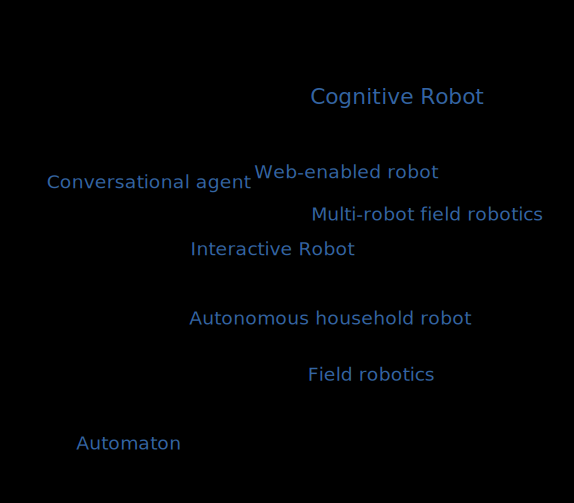
\includegraphics[width=0.7\columnwidth]{intro/social_skills.pdf}
    \caption{Towards the cognitive robot}
    \label{fig|cognitive-robots}
\end{figure}



\begin{itemize}
    \item to loosen the constraints on symbolic modeling of the robot
    environment by providing more expressive representation system than
    classical databases or fact repositories,

    \item to improve human-robot interaction by explicitly providing to the
    machine an interpretation frame, at least partially shared with the human.

\end{itemize}


%%%%%%%%%%%%%%%%%%%%%%%%%%%%%%%%%%%%%%%%%%%%%%%%%%%%%%%%%%%%%%%%%%%%%%%%%%%%%%%
%%%%%%%%%%%%%%%%%%%%%%%%%%%%%%%%%%%%%%%%%%%%%%%%%%%%%%%%%%%%%%%%%%%%%%%%%%%%%%%
%%%%%%%%%%%%%%%%%%%%%%%%%%%%%%%%%%%%%%%%%%%%%%%%%%%%%%%%%%%%%%%%%%%%%%%%%%%%%%%

\section{A prototypical scenario}
\label{sect|scenario}

\begin{figure*}
	\centering
	\includegraphics[width=0.9\textwidth]{intro/brownie_scenario.jpg}
	\caption{An illustration of the scenario}
	\label{fig|scenario}
\end{figure*}

The aim of this imaginary scenario (that has not been implemented, neither in
simulation nor on a robot) is to materialise early in this thesis the context
and challenges of knowledge representation and manipulation for service, social
and interactive robotics. It underlines the place, the role and the need of
knowledge in a near-future, everyday situation where several robots and humans
co-exist and cooperate. This scenario will also be a source of support examples
for later sections of the thesis.

We entitle our scenario ``the Brownie scenario'' (Figure~\ref{fig|scenario}):
Robi and Roba are two service robots, that can freely
move and pick objects around (with possibly different hardware and softwares
architectures, including different knowledge representation systems). They
cooperate with a human in a kitchen environment.

The main task of the scenario is the joint realization of a brownie, initiated
by Tom, the human: ``Let's make a brownie for tonight!''.

The scenario is successful if the task is achieved (the brownie is baked) in a
reasonable time (typically shorter than what it would have been required by the
human alone).

We voluntarily do not detail the subtasks of the scenario, neither we define
how they are shared amongst agents: our focus is on knowledge needs and flows.

A ``first-order'' analysis of this task leads to a rough partition of the
required \emph{representation} abilities:

\begin{enumerate}

	\item Representation abilities related to the execution of a complex
	spatio-temporal task,

	\item Representation abilities related to cooperation with other agents.

\end{enumerate}

% Representation of a complex task
We can further refine these categories: to prepare and bake a brownie, the
robot first needs to make sense of the term \emph{brownie} itself: what is it?
what is it used for? what is it made of? etc. We call this knowledge
\emph{common-sense knowledge} and the robot must be able not only to represent
it, but also to have access to an initial source (for instance through a
initial set of facts that are made available at startup, or via access to a
Web-based knowledge base like Wikipedia, etc.)

Once bound to the action \emph{make}, this should lead the robot to build and
represent a \emph{context}: we are in a scenario involving cooking. The context
enables the robot to retrieve more common-sense knowledge, like that actions
related to cooking often take place in the kitchen, cooking requires
ingredients, utensils and a procedure that may be provided by a recipe.

These last assertions imply several other capabilities: ``cooking often takes
place in the kitchen'' implies that representation of both uncertainty and
likelihood is desirable. The fact that cooking is associated to a place further
implies that the system models locations and is able to attach \emph{thematic
relations} to concepts (here, the likely location of the cooking action).

``cooking requires ingredients'' hints about another important feature closely
tied on knowledge manipulation: \emph{reasoning}. The robot can \emph{infers}
that cooking may require a recipe since a list of ingredients is a
pre-requisite of the cooking action, and a recipe may provide such a list.  If
we omit the ``may'', this is a typical example of first-order logic reasoning.
Many other reasoning techniques exist (including probabilistic ones -- ones
able to deal with the ``may''), we shall illustrate some of them later in this
scenario.

We mentioned that a recipe often provides a procedure (or a \emph{plan}). The
robot should be able to store this plan in a way that allow later execution.
The plan is likely to contain \emph{spatio-temporal constraints} (like ``put
the brownie in the oven for 20 min'' or ``let's cook \emph{for tonight}'') that
must be as well appropriately handled.

To make decision, a robot may also want to \emph{predict} the state of the
world after some action (``if I leave the cake 2h in the oven, it will burn'').
Such ability to project itself in future or, generally speaking, in other
possible state of the world is related to several cognitive ability and
reasoning techniques: \emph{planning}, \emph{projection}, \emph{representation
of possible worlds} and \emph{non-monotonic reasoning}, in addition to
common-sense knowledge and \emph{physics-based} reasoning (that allows for
instance to predict that an egg is likely to break if dropped).

Procedures are in addition often \emph{underspecified}: we can expect the
recipe to provide a cooking duration, but we usually do not expect the recipe
to tell us to first open the oven door, and then put the cake into it, since it
is self-evident that the door must first be opened to put the cake in the oven.
Our cognitive robot should ideally be able to detect and possibly complete such
underspecification.

% Representation feature that enable cooperation
Then, we want our three agents to cooperate. This, in turn, leads to another
set of cognitive abilities.

Cooperation in our scenario can intervene at many places. For instance, an
agent may want to inform another one about the number of eggs that are
necessary for the brownie. This \emph{helping} behaviour makes sense only if
the first agent knows that the recipient agent both needs the information but
does not know it. This in turn requires the robot to be able to model the
knowledge of the other agents: to think \emph{from the perspective} of another
agent (an idea that is related to the availability of a theory of mind, we will
come back to it later on).

Ability to communicate is one important pre-requisite to collaboration.
Communication in general requires the addresser and the addressee to share a
common interpretative framework (a shared common-sense knowledge -- or cultural
background -- and a shared context). In our scenario, the agents are working in
a kitchen. This element of context does not however suffice if, for example, an
agent asks another agent to ``give {[him]} the bowl''. Behind the symbol
``bowl'', which physical entity are we actually talking about? If we want to
talk and act on the world, this so-called \emph{grounding} operation is
essential. It is a bidirectional process: in covers the {\it top-down}
operation (from the symbol to the percept) and the {\it bottom-up} converse
(retrieval or creation of symbols from perception).

A related ability is called \emph{pre-supposition accommodation}: if one of the
agent moves behind another one, with the brownie dough in its arm, and says
``be careful, I'm behind you!'', we want the first agent to be able to
represent both symbolically and geometrically (because, for instance, if the
agent want to move, it must take into account the new obstacle) something that
is not directly perceived.

Also central to cooperation are the notions of \emph{joint intentions} and
\emph{joint goals}: to help the human during the cooking session, the robots
need to track how far they are into the recipe, what is the next step the human
is likely to go for, how task are currently split between agents, what action
is currently blocking the procedure, etc. This knowledge should let the robot
identify the intentions of other agents and create accordingly joint goals.
Hence, a knowledge representation system aiming at dealing with cooperative
behaviours is likely to have goal management structures taking explicitly into
account other agents' actions and goals.

In order to effectively share tasks, the robot must also know what it is
capable of: \emph{capability introspection} (both in term of general capability
and of immediate ability) is thus often desirable. It can be extended to
general introspection (like the ability to tell ``who I am'' or ``what do I
think of'') that may be required for the interaction.

Last but not least, our scenario assumes implicitly \emph{natural interaction}
between humans and robots (as showed by the casual style of the order ``Let's
make a brownie!''), and we want to ensure that the
knowledge available to the robot provides efficient support to the natural
language understanding (for instance by adopting models and vocabulary that are
both well suited for machine processing and remain as close as possible to the
humans own structures and vocabulary), and also to \emph{non-verbal forms of
communication}, like gestures.


We have emphasised several keywords in this scenario: we will come back to them
in chapter~\ref{chapt|krs} to explain them formally, and relate them to each
other. Before that, we would like to briefly focus on the challenges
specifically related to the human-robot interactions. Not only in term of
knowledge representation, but more broadly in term of specific cognitive
capabilities.

%%%%%%%%%%%%%%%%%%%%%%%%%%%%%%%%%%%%%%%%%%%%%%%%%%%%%%%%%%%%%%%%%%%%%%%%%%%%%%%
%%%%%%%%%%%%%%%%%%%%%%%%%%%%%%%%%%%%%%%%%%%%%%%%%%%%%%%%%%%%%%%%%%%%%%%%%%%%%%%
%%%%%%%%%%%%%%%%%%%%%%%%%%%%%%%%%%%%%%%%%%%%%%%%%%%%%%%%%%%%%%%%%%%%%%%%%%%%%%%

\section{Robots for interaction}
\label{sect|hri-context}

This work comes indeed from researches in the specific context of the
human-robot interaction, or, to put it another way, in the context of
interaction for \emph{joint action} with human,  in a \emph{situated}
environment (figure~\ref{fig|aperitif}).

\begin{figure}%[!ht] 
    \centering
    \includegraphics[width=0.8\columnwidth]{intro/aperitif_time.jpg} 

    \caption{Interacting with the robot in an everyday situation: the human
    asks for help in vague terms, the robot takes into account the human's {\it
    a priori} knowledge and spatial perspective to refine its understanding of
    the question.} 

    \label{fig|aperitif} 
\end{figure}

{\em \emph{Let's bake a brownie for tonight!}, proposes Tom. The robots
smoothly prepare all the ingredients, and they start to cook together a
delicious cake...}

Natural interaction and cooperation are actually the current (dare we say,
\emph{short-term}) targets for the human-robot interaction community.  The
``Brownie scenario'' we presented above belongs to the broad class of
\emph{interactive manipulation problems}: several agents agree on a (more or
less implicit) joint goal that requires some sort of cooperation to be
successfully achieved. This class of problems involves both dialogue and
manipulation and is often not completely defined at start-up: it requires
iterative, interactive resolution (step-by-step process,
questions-answers,...).

What are the cognitive prerequisites for such a sentence --``Let's make a
brownie for tonight''-- to be understood by the robot, correctly interpreted in
the spatial and temporal context of the interaction, and eventually transformed
into a set of actions? We distinguish~\cite{Lemaignan2012} four successive
steps:

\begin{enumerate}

    \item how to build and maintain a consistent geometric model of the current
        situation, acquired through perception or deduction from previous
        perceptions,

    \item how to build an unambiguous symbolic representation of concepts
        (objects, agents, actions...) underlying the interaction, and practical
        for decision-making processes,

    \item how to establish the joint goal(s), how to build and maintain
        iteratively shared (human-robot) plans, 

    \item how to refine and execute the computed plans, and how to monitor
        those achieved by its human partner?

\end{enumerate}

This work focuses on the second point: it presents techniques, developed and
used on several real robots, for the symbolic representation of environment
models suitable for grounded situation interpretation, decision-making and
control.

The other items are of course equally important to actually perform the
interaction, and we will also present (and illustrate in experiments) how our
knowledge representation system integrates and communicates with other
processes to form a \emph{knowledge-enabled} robotic architecture.


\begin{figure}
    \centering
    \includegraphics[width=0.9\columnwidth]{intro/grounding_robot.pdf}
    \caption{A robot reasoning about human-robot interaction and anticipation
    of human activities: sources of knowledge are multi-modal dialogue and
    observation of the environment and the human activities.}
    \label{fig|hri-dec}
\end{figure}


Figure~\ref{fig|hri-dec} summarises the main aspects of the interaction.
From the robot perspective, several cognitive skills are involved: dialogue
processing through verbal and deictic modalities (what does the human say? What
attitude -- glances, postures, gestures... -- does he express?), acquisition
and maintenance of one or several models of the environment, not only from the
robot point of view, but also from the other agents' points of view,
anticipation (what are the intentions of the human? Can I predict and
anticipate his/her actions?), planning and control (how would I proceed further
towards the goal?), monitoring of the other agents' activities (do we have an
effective cooperation?) and the overall progress of the task. 

As we shall see, all these cognitive capabilities also translate into
requirements on the knowledge representation systems that we want to clarify.

\begin{figure}%[!ht]
\centering
  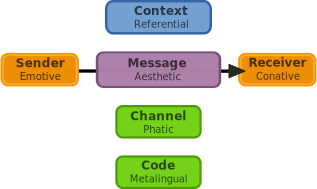
\includegraphics[width=0.6\linewidth]{communication/jakobson_communication_model.pdf}

  \caption{The \emph{Communication Model}, as proposed by
  Jakobson~\cite{Jakobson1960}. In bold characters are the \emph{communication
  dimensions}, in italics, the corresponding \emph{communication functions}.}
  
  \label{fig|jakobson_communication_model}
\end{figure}


The need of communication is probably the most salient one. The classical model
of communication proposed by Jakobson in 1960
(figure~\ref{fig|jakobson_communication_model}) exposes in a bright way the
main functions involved in a communication, be it verbal or non-verbal. While
the \emph{channel} and the \emph{code} are the technical side of the
communication, the \emph{message} in relation with the \emph{context} are
directly concerned with the question of the \emph{meaning} which itself as
tight links with the knowledge available to the agent.

The question of the communication between a robot and another agent (in a broad
way: another robot, an human, but also a remote knowledge base or the robot's
developer) underlies many of the challenges of knowledge representation: how to
represent the knowledge I want to exchange, and how to recognize, represent and
share a context that ensures both the end of the communication channel
correctly interpret the message. Or, to put it another way: how to ensure the
\emph{meaning} is correctly carried around while conducting social
interactions.

%%%%%%%%%%%%%%%%%%%%%%%%%%%%%%%%%%%%%%%%%%%%%%%%%%%%%%%%%%%%%%%%%%%%%%%%%%%%%%%

\section{The Challenges}
\label{sect|challenges}

From the set of questions raised in the previous paragraphs, we can now
articulate the challenges that are to be tackled in this field of knowledge
representation for service/companion robotics.

The first challenge is to... clarify the challenges (!) of knowledge
representation: we say ``knowledge'', we say ``reasoning'', we say
``representation'', but clear definitions are yet to be provided. Numerous
requirements on what Newell calls the \emph{knowledge level} of intelligent
agents have emerged from our \emph{Brownie} scenario, but how do they
articulate? And are they comprehensive?

To further develop what is widely known as the ``cognitive robotics'', we think
it is mandatory to lay down solid theoretical and practical foundations to the
knowledge needs of service/interactive robots. This is our first challenge.

The second challenge is more technical: how to build such a
``knowledge-enabled'' robot? Since many years, research has started to create
and study so-called cognitive architectures. Robots, as embodied and
interactive agents, raise specific issues. What are they? Which are the right
technical approaches? Can we build today such a cognitive system, and if we can
not, why that? How the abstract idea of knowledge translates into  practical,
meaningful concepts?

Our third challenge relates to the specific question of the human-robot
interaction: the robot enters the realm of a social individuality. What does
that mean? Which consequences does that have on our initial knowledge
challenge? How does it translate into practical issues, like natural language
understanding?

All the contributions (summarised in the next section) of this thesis can be
related to one of these three challenges, and hopefully contribute to the
advancement of the understanding of these questions.

%%%%%%%%%%%%%%%%%%%%%%%%%%%%%%%%%%%%%%%%%%%%%%%%%%%%%%%%%%%%%%%%%%%%%%%%%%%%%%%


\section{Contributions}
\label{sect|contributions}

We have presented our challenges: this section now summarises the main
contributions of the thesis, both from a scientific point of view and from a
technical point of view.

\subsection{Scientific contributions}
\label{sect|scientific-contributions}

The need of a better understanding of the knowledge needs of robotic
applications in human, \ie complex, dynamic, semantically-rich, environments,
is the starting point of our thesis.

Building upon an extensive review of the literature and the formulation of
several interaction scenarii (that themselves led to experiments on real
robots), we have iteratively refined the ``knowledge for interaction'' problem.
The formalization of this question is one of the main scientific outcomes of
this work: we have listed and organized into a typology a set of desirable
characteristics of knowledge representation systems for service robotics.

This typology aims at offering a comprehensive and consistent base to evaluate
existing systems and to draw new research perspectives. It also enables to
better assess the progresses of the Service Robot and Human Robot Interaction
research communities towards the long term goal of \emph{human-level artificial
intelligence} for robots, as would say McCarthy.

Another scientific contribution of this thesis is its participation to
narrow down the gap between research on embodied and disembodied artificial
agents: we have tried to bridge experiences learned from years of research on
disembodied cognitive architectures (both from the computing science and
neuropsychology communities) with the constraints from real-world systems that
weigh on robotic architectures. Notably, we have tried to identify
theoretical reference contributions from the diverse fields of cognitive
sciences that are relevant to \emph{knowledge-enabled} robotics. We have also
proposed reference implementations on robots for some of them.

At the architectural level, our work also helps to better understand the
knowledge flows in modern cognitive architectures for robots. By introducing
\emph{explicit} knowledge in our architectures, it allows the humans that
design and program robots to \emph{talk about} and question this knowledge: it
singularises and materialises concepts that were beforehand often
diffuse and ubiquitous. This leads us to define the idea and propose an
implementation of a \emph{knowledge-oriented} architecture.

This work has also several more focused scientific contributions. The
centralized semantic architecture that we propose is original. While it
exhibits shortcomings for some cognitive tasks, it also proposes novel efficient
ways to represent and manipulate knowledge simultaneously for multiple agents.
Along with the survey of current knowledge systems that we have conducted,
it effectively completes the panorama of available designs of knowledge
representation systems.

Amongst the cognitive abilities that our developments have enabled, a
particular scientific focus was led on the acquisition and modeling of
multiple, agent-dependent symbolic worlds. This opened new perspectives related
to \emph{perspective-aware} reasoning or \emph{theories of mind} for robots
that are detailed in this work.

We also have a scientific contribution on the grounding of human-robot
dialogue in natural language. We have algorithmically formalized a novel
grounding process that takes advantage of multi-modal communication (verbal,
deictic and immanent) and handles the semantics of several more complex
language features like quantification. This system also has contributions
related to the semantic validation of thematic roles and interactive
disambiguation that takes into account human attentional focus.

\subsection{Technical contributions}
\label{sect|technical-contributions}


This thesis has four major technical contributions: the software development of
\emph{ORO server} as a semantic blackboard dedicated to robotic applications,
the design of the \emph{ORO ontology} as a domain-specific common-sense
ontology tailored for service robotic needs, the pervasive integration of a new
semantic layer into several existing robot architecture, and finally, the
software development of \emph{Dialogs}, a novel module for natural language
grounding.

The main software contribution of the thesis is the development of an
open-source, versatile and light-weight knowledge base that stores in a
formal framework based on first-order logics both the robot's own beliefs and
the mental models of every other cognitive agents that the robot interacts
with. This tool, called \emph{ORO}, is implemented as a
platform/middleware-agnostic server, and exposes to the robot's modules
several advanced reasoning services (via the integration of external
reasoners). This software project is now publicly available, used by other
laboratories, and comes with extensive documentation and bindings for several
mainstream languages (C++, Python...) and middlewares (ROS, YARP).

In parallel of this development, and in collaboration with other developers,
we have also drafted (and partially implemented) a proposal for a standard API
for knowledge manipulation that supports the specific needs of robotic
applications.

Coming along with the ORO server, we introduce in this thesis the
\emph{ORO common-sense ontology} which is a proposal of an upper ontology for
service and interactive robotics. This ontology consists of about two hundred
classes, relations and rules that are relevant for the modeling of the
robot's beliefs and state, and the interactions with other agents (humans or
robots). This ontology also tries to stay closely aligned with the standard
{\sc OpenCyc} upper-ontology to guarantee interoperability with semantic
web resources and other robots.

A third technical contribution is the introduction of a new
knowledge-oriented, event driven communication model between high-level
decisional modules: by introducing the concept of \emph{semantic events}, the ORO
server enables the development of new executive layers that combine reactive
behaviour with high-level abstractions: for instance, triggering a behaviour
when a human looks at the robot while sit, can be expressed in our architecture
as a single proposition: {\tt subscribe([* type Human, * looksAt myself, *
isSitting true], behaviour\_callback())}. This highly expressive event model
opens new ranges of development opportunities for decisional modules.

During the preparation of the thesis, we have also developed a new stand-alone
natural language processor for English language. It takes advantage of the
different symbolic models exposed by the ORO server to analyse, resolve the
semantics and ground dialogues. It can process orders, questions and positive
assertions and translates them into new symbolic facts. It includes a custom
grammatical parser, a re-verbalization module, several discrimination
strategies, including interactive ones. The application is developed in Python
(about 15K lines of code), can be used in real-time on the robot, and is
accompanied by a speech recognition interface developed as an Android
application.

A last notable software contribution is our involvement in the MORSE simulator
for academic robotics. We have played a central role in the original design and
development of the core functionalities of this open-source simulator which is
now used by over twenty laboratories world-wide. While this project as a whole
is not directly related to the thesis main domain, we have led the effort towards
effective simulation of human-robot interaction in MORSE, which is now the
current state-of-the-art in this domain. It is briefly presented at
section~\ref{sect|simulation}.


%%%%%%%%%%%%%%%%%%%%%%%%%%%%%%%%%%%%%%%%%%%%%%%%%%%%%%%%%%%%%%%%%%%%%%%%%%%%%%%
%%%%%%%%%%%%%%%%%%%%%%%%%%%%%%%%%%%%%%%%%%%%%%%%%%%%%%%%%%%%%%%%%%%%%%%%%%%%%%%
%%%%%%%%%%%%%%%%%%%%%%%%%%%%%%%%%%%%%%%%%%%%%%%%%%%%%%%%%%%%%%%%%%%%%%%%%%%%%%%


\section{A reader's guide}

\subsection*{The thesis in 15min}

Because of the contingencies of this world, we acknowledge that the complete
reading of this thesis may not fit in one's tight schedule.

If you have only about 15 minutes to dedicate to this work, we suggest to read
the following sections in that order:

\begin{itemize} \item What are the challenges? (section~\ref{sect|challenges},
            page~\pageref{sect|challenges}),

    \item Contributions (section~\ref{sect|contributions},
        page~\pageref{sect|contributions}),

    \item The ORO functional overview (section~\ref{sect|functional-overview},
        page~\pageref{sect|functional-overview}),

    \item The first interaction experiment (section~\ref{sect|expe1},
        page~\pageref{sect|expe1}),

    \item The evaluation of ORO and other knowledge representation systems
        (section~\ref{sect|evaluation-oroserver},
        page~\pageref{sect|evaluation-oroserver}),

    \item And finally, the discussion on perspectives
        (section~\ref{sect|perspectives}, page~\pageref{sect|perspectives}),

\end{itemize}

Hopefully, this quick overview of this work can help you to go in depth into
the sections relevant to your concerns.

\fxfatal{Re-read these sections to make sure it makes sense}

\subsection*{For the patient reader}

Roughly speaking, the thesis is organized in three parts: an analysis of
knowledge representation systems for service and personal robotic, the
presentation of ORO, our own implementation of such a knowledge representation
system, and finally we report on practical uses of explicit knowledge
manipulation on robots, first for natural language processing, then through
several experiments.

The first part is covered in the chapter~\ref{chapt|krs}: after a discussion on
what we call ``knowledge'' in our context, we explore its importance by
listing, in a typology of characteristics, the requirements of our robots
related to knowledge management. This first chapter is completed by a survey of
eight systems for knowledge management that have been already deployed on real
robots.

At the end of the thesis, we give a second look at these systems to try to
draw a picture of the overall landscape of knowledge representation approaches
in the robotic reseach community, to identify new possible research directions.

The second part is covered by chapters~\ref{chapt|oroserver} and
\ref{chapt|implementation-integration}. Chapter~\ref{chapt|oroserver} presents
the functional side of ORO server, some of the algorithms that are
implemented, and discusses its knowledge model (the ORO \emph{common-sense
ontology}). The technical side is presented in
chapter~\ref{chapt|implementation-integration} where we emphasise the
integration of ORO within a larger robotic architecture. The articulations with
perceptions, planning and control are presented.

Chapters~\ref{chapt|dialogs} and \ref{chapt|evaluation} form the third and last
part of the thesis. Chapter~\ref{chapt|dialogs} details \emph{Dialogs}, a
module for situated dialogue grounding that takes advantage of the symbolic
knowledge exposed by ORO, and chapter~\ref{chapt|evaluation} presents
several evaluations of our work through various experiments conducted during
the four years of the thesis preparation.

We conclude the thesis with a discussion of several issues related to knowledge
management in service robots (importance of embodiement, relationships between
the symbolic and continuous realms, etc.) and some remarks that could further
improve knowledge representation and management in future robotic
architectures.


\chapter{Symbolic knowledge representation}

\section{Which end for knowledge representation?}
\label{sect|krs-purpose}

\subsection{Limits of traditional representation systems for robotics}
\label{subssect|limits}

\subsection{Specific requirements of robotics}
\label{subssect|robotics-specifics}

\subsection{Benefits of a symbolic knowledge representation system}
\label{subssect|krs-benefits}

\section{Formalisms for symbolic representation}
\label{sect|formalisms}

\section{Designing the \textsc{OpenRobots} common-sense ontology}
\label{sect|commonsense-design}

\section{Evaluation of a symbolic representation }
\label{sect|krs-evaluation}


\chapter{oro-server, a symbolic knowledge representation system for robotics}
\label{chapter|oroserver}

This chapter introduces the \emph{OpenRobots Ontology} server and its
common-sense knowledge base.

We present a \textbf{functional description} of oro-server, and detail at
lenght its knowledge model. Its actual implementation is discussed in the next
chapter.

We also present in depth the \emph{OpenRobots Common-Sense Ontology} that
contains most of the knowledge at hand when the robot starts.

\section{Functional overview}
\label{sect|functional-overview}


We have adopted a centralized approach for knowledge management called
ORO~\cite{Lemaignan2010}. The platform is designed as a central
knowledge storage service implemented as a server where the robot
components can add or query statements at run-time. Figure~\ref{fig|oro-overview}
illustrates the main functional components of ORO.

\begin{figure}
\centering
  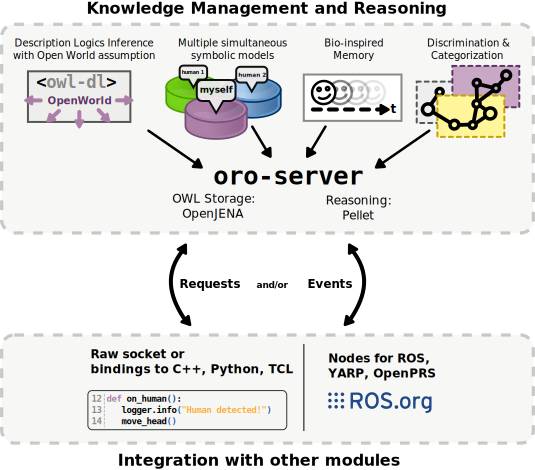
\includegraphics[width=0.8\linewidth]{oroserver/oro_architecture_functional.pdf}
  \caption{Overview of the ORO architecture.}
  \label{fig|oro-overview}
\end{figure}

At the core, ORO is build around the
OpenJena\footnote{\url{http://www.openjena.org}} ontology management library,
connected to the Pellet\footnote{\url{http://clarkparsia.com/pellet}}
reasoner.

A front-end accepts and manages connections to clients. The clients' requests
are processed by a set of internal modules: basic operations on statements,
but also higher cognitive and human-robot interaction related functionalities
are available. External plugins can also be easily added.

Besides acting as a facts database, the ORO platform exposes several
functions: operations on knowledge statements relying on inference (through a
continuous first-order logic classification process), management of
\emph{per-agent} symbolic models, and also higher cognitive and human-robot
interaction related functionalities like categorization of sets of concepts
or profiles of memory (that enable the robot to ``forget'' about some facts).

ORO also provides an event mechanism that allows components to be triggered
when specific events occur. A component can for instance subscribe to events
of kind \setstmt{?agent isVisible true, ?agent type Human}. As soon as the
perception layer detects a human in the robot's field of view and accordingly
updates the knowledge base, the executive layer is triggered. The event
framework also takes advantage of the inference capabilities of ORO. Thus an
event can be indirectly triggered if its triggering conditions can be
inferred to be true.


%%%%%%%%%%%%%%%%%%%%%%%%%%%%%%%%%%%%%%%%%%%%%%%%%%%%%%%%%%%%%%%%%%%%%%%%%%%%%%%
%%%%%%%%%%%%%%%%%%%%%%%%%%%%%%%%%%%%%%%%%%%%%%%%%%%%%%%%%%%%%%%%%%%%%%%%%%%%%%%
%%%%%%%%%%%%%%%%%%%%%%%%%%%%%%%%%%%%%%%%%%%%%%%%%%%%%%%%%%%%%%%%%%%%%%%%%%%%%%%

\section{The ORO Knowledge model}
\label{sect|knowledge-model}

\subsection{Expressiveness: What Can be Represented?}
\subsubsection{Open World and Close World Assumptions}
\subsubsection{Meta-cognition: knowledge on the knowledge}
Narrower, more technical dimension of the introspection.

%%%%%%%%%%
\subsection{How things are represented?}
\subsubsection{Role Representations}
Spatio-Temporal Representations:

\paragraph{Representation of time}
\paragraph{Representation of space}
\paragraph{Representation of events and actions}

\subsubsection{Context modeling}
\subsubsection{Possible-Worlds and representing what others know}

\paragraph{Multi-model representation for Persepective-taking}
\label{sect|alterite}

...

We present at section~\ref{sect|perspectivetaking}, page~\pageref{sect|perspectivetaking} an 3D real-time environment, SPARK, that allows to compute on-line several perspective aware symbolic properties.

\subsection{False beliefs and Theory Of Mind}
\label{sect|theory-of-mind}



\subsubsection{Introspection: Who am I? What can I do?}

%%%%%%%%%%
\subsection{Reasoning Techniques}

\subsubsection{Standard reasoning techniques}


Knowledge is stored as OWL/RDF ontologies in ORO. We use the Pellet reasoner to
classify them. This enables several type of reasoning:

\begin{itemize}
	\item reasoning on inheritance relations (\eg \emph{all bottles are containers}),
	\item property axioms
		\begin{itemize}
		\item entailments based on predicates' domain and range,
		\item cardinality constraints (including \concept{allValue}, 
		\concept{someValue}, \concept{hasValue}),
		\item property characteristics (symmetry, transitivity)
		\end{itemize}
	\item class restrictions like: \par \footnotesize \concept{Bottle} $\equiv$
		\concept{Artifact} {\bf that} (\concept{hasShape} {\bf value}
		\concept{cylinderShape})\footnote{This example uses the \emph{Manchester
		syntax}, \url{http://www.w3.org/TR/owl2-manchester-syntax/}} \normalsize
	\item set operations like: \par \footnotesize \concept{Color} $\equiv$ {\bf unionOf}(\concept{blue},
		\concept{green}, \concept{orange}, \concept{black}...) \normalsize
	\item generic SWRL ({\em Semantic Web Rule Language}) rules like: \par
		\footnotesize \concept{looksAt(?agt, ?obj)} $\land$
		\concept{pointsAt(?agt,?obj)} \par $\Rightarrow$ \concept{focusesOn(?agt, ?obj)}
		\normalsize 
	\end{itemize}

We provide in ORO accessors to query, add or remove all these properties and
restrictions (except the SWRL rules) at run-time. This allows knowledge
introspection and enables the robot to alter its own knowledge structures (the
so-called \emph{T-Box} model) during its life-time by adding new constraints
and properties to classes and predicates (we can for instance teach the robot
\emph{at runtime} that cats are animals, \ie \stmt{Cat rdfs:subClassOf
Animal}).


\paragraph{Decidability}

...


\subsubsection{Reasoning with uncertainty}
\subsubsection{(Non) Monotonic Reasoning}


\subsubsection{Memory}
\label{subssect|memory}


\subsubsection{Learning by modifying the knowledge structure}

%%%%%%%%%%%%%%%%%
\subsection{The left-overs: What ORO does not provide?}

\subsubsection{Representation of uncertainty and likelihood}

\subsubsection{Presupposition accommodation}
\subsubsection{Prediction, projection and diagnosis tasks}
\paragraph{Projection task}: determining whether or not some condition while
hold after a sequence of actions.

\paragraph{Legality task}: determining whether a sequence of action can be
performed starting in some initial state.

\paragraph{Diagnosis}: this corresponds to the ability to rewind on past events
in case of failure to provide possible explanation. This can be seen as the
temporal reverse of the projection task.


\subsubsection{Physics-based reasoning}
\subsubsection{Planning}
Making decision based on prediction




%%%%%%%%%%%%%%%%%%%%%%%%%%%%%%%%%%%%%%%%%%%%%%%%%%%%%%%%%%%%%%%%%%%%%%%%%%%%%%
%%%%%%%%%%%%%%%%%%%%%%%%%%%%%%%%%%%%%%%%%%%%%%%%%%%%%%%%%%%%%%%%%%%%%%%%%%%%%%
%%%%%%%%%%%%%%%%%%%%%%%%%%%%%%%%%%%%%%%%%%%%%%%%%%%%%%%%%%%%%%%%%%%%%%%%%%%%%%

\section{Knowledge instanciation: the OpenRobots Common-Sense Ontology}

How much knowledge is available? Which content? How big is the knowledge base?

\subsection{Designing the \textsc{OpenRobots} common-sense ontology}
\label{sect|commonsense-design}



\chapter{ORO Implementation and integration in robots}
\label{chapter|implementation_integration}

\section{Some implementation notes}

This section presents some of the main technological choices that have
been made to implement the knowledge base.

Some of the main algorithms are presented here as well (like the algorithms for clasification and discrimination,~\ref{sect|discrinimation}).

\subsection{A centralized server-based implementation}
\label{sect|oro-serverbased}


\subsection{OWL-DL ontologies and Jena}
\label{sect|jena}

\subsection{Reasoning: the Pellet reasoner}
\label{sect|pellet}

\subsection{Classification and discrimination algorithms}
\label{sect|discrimination}

\section{Bindings to other components/languages}
\label{sect|interfacing}

%%%%%%%%%%%%%%%%%
\section{Integration in the robot architecture}

\subsection{RPC and events-oriented interactions}

\subsection{Acquiring Knowledge}

\subsubsection{Knowledge acquisition and modalities merging}

\paragraph{Perception}
\paragraph{Interaction}
\paragraph{External sources (Web, upper ontologies, ...)}
\paragraph{Learning}

\subsubsection{Perspective taking}
\label{sect|perspectivetaking}

\subsubsection{Grounding/anchoring strategies}

\subsubsection{Ability to automatically create new object instances}

%%%%%%%%%%%%%%%%%

\subsection{Integration with symbolic task planning and executive layers}

\fxnote{CRAM, SHARY, pyrobots...}

\subsection{Integration with natural language processors}


\subsubsection{Monitoring and debugging}

\subsubsection{Is it fast enough? Scalability and responsiveness}



\chapter{An advanced application: situated natural language processing}
\label{chapter|dialogs}

%%%%%%%%%%%%%%%%%%%%%%%%%%%%%%%%%%%%%%

\section{Grounding human interaction into the robot knowledge}
\label{sect|dialogs}

\subsection{Situated speech acts}
\label{intro_example}

A messy table, covered with cardboard boxes, books, video tapes... Thomas is
moving and packs everything with the help of Jido, its robot.

`` -- Jido, give me this'', says Thomas, looking at a box that contains a video
tape. The robot smoothly grasps the tape, and hands it to the human.

While this kind of interaction should hopefully sound quite familiar in a
foreseeable future, our robots are not yet quite up to the task. Neither
regarding natural language understanding nor plan-making and manipulation.

To be combined together, those abilities require an unambiguous and shared
representation of concepts (objects, agents, actions...) underlying the
interaction: what are the prerequisites for such a
human sentence --- ``Jido, give me this'' --- to be understood by the robot,
correctly interpreted in the spatial context of the interaction, and ultimately
transformed into an action?

Austin~\cite{Austin1962} would have at first glance analyzed such kind of
sentence as a \emph{speech act}, comprising of \emph{locutionary},
\emph{illocutionary} and possibly \emph{perlocutionary} acts. First, we want to
understand the direct meaning of the sentence (\emph{locutionary act}): we must
acquire the sentence, convert it into a useful syntactic form (quite probably
by mean of speech recognition), and understand the semantics of the sentence,
\ie, What is refered by ``\textit{Jido}''? What is ``\textit{give}''? What is
``\textit{me}''? And ``\textit{this}''?

Working in a situated context, we want furthermore to \emph{resolve} these
semantics atoms, \ie ground them in the sensory-motor space of the robot. For
instance, ``\textit{this}'' is a demonstrative pronoun that refers in this
context to the object the human is focusing on, whatever \textit{focusing}
means: here, Thomas is looking at something, which is a possible cue. But it
could as well point at something or refer to some previously mentioned concept. 

\begin{figure}%[!ht] 
	\centering
	\includegraphics[width=0.9\linewidth]{images/dialogs/pt.jpg} 
	\caption{Interacting with
	the robot in an everyday setup: the human asks for help in vague terms, the
	robot takes into account the human's spatial perspective to refine its
	understanding of the question.} 
	\label{fig|vpt} 
\end{figure}


Second, the \emph{illocutionary force}, \ie the \emph{intent} of the utterance
as thought by the agent must be extracted, and understood. In our example,
Thomas obviously wants an action to be performed by the robot. The action
parametrization is conveyed by the semantics attached to the words and the
grammatical structures of the sentence. In our example, the type of action is
given by the verb ``\textit{give}''. Assuming the robot has some procedural
knowledge attached to this symbol, the action type can be considered as
grounded for the robot. We can as well understand that the recipient of the
action is the human, the performer is the robot itself, and the object acted
upon is the tape. These are the basic \emph{thematic roles}~\cite{Gruber1965}
that can be extracted from the sentence that allow to fully ground the action.

\subsection{Building a symbolic model}

Extracting these speech acts and turning them into a content processable by the
robot is a difficult challenge in the general case. We base our approach on
three distinct, inter-related cognitive functions:

\begin{inparaenum}[\itshape 1)]

\item \emph{Physical environment modeling} and \emph{spatial reasoning}
(grouped under the term \emph{situation
assessment})  are in charge of building and
maintaining a coherent model of the physical world. This model is realistic in
the sense that it relies on accurate 3D models of both manipulated objects and
humans. It also has dedicated mechanisms to manage disappearing or occluded
objects.  The geometric model is used to compute several spatial properties of
the scene that actually convert the original sensory data into symbolic
beliefs. This includes relative locations of objects, visibility state,
gestures like pointing, etc.  Assuming that other agents are as well
represented in the model, the same computations are applied to analyze the
scene from each agents' point of view (\ie from their \emph{perspectives}).
This approach is presented in depth in~\cite{Sisbot2011}.

\item \emph{Knowledge representation and management}: the robot is endowed with
an active knowledge base that provides a logically sound symbolic model of its
beliefs on the world, as well as models for each cognitive agent the robot
interacts with. Each of these models is independent and logically consistent.
This enable reasoning on different perspectives of the world that would be
considered otherwise inconsistent (for instance, an object can be visible for
the robot but not for the human. This object can have at the same time the
property {\tt isVisible \textbf{true}} and {\tt isVisible \textbf{false}}, in
two different models).  Our platform also features continuous storage, querying
and event triggering over the pool of facts known by the robot. It relies on
OWL ontologies (a decidable subset of the predicate logics). The knowledge base
is presented in~\cite{Lemaignan2010}.

Used in combination with the situation assessment framework, the robot is thus
able to maintain different models of the world, one per agent. This proves an
essential feature (\cite{Roy2005, Kruijff2010}) to enable perspective-aware
grounding of natural language, as we will see in next sections.

\item \emph{Dialogue input processing}, including natural language parsing
capabilities, disambiguation routines and interactive concept anchoring. We
focused our efforts on three classes of utterance, commonly found in
human-robot interaction: \emph{statements} (\ie new facts the human wants to
inform the robot), \emph{orders} (or more generically \emph{desires}) and
\emph{questions on declarative knowledge} (whose answers do not require
explicit planning). This would roughly cover the \emph{representative}
(sometimes referred as \emph{assertives}) and \emph{directives} type of
illocutionary acts, in Searle~\cite{Searle1976} classification. This paper
focuses on this last facet (dialogue processing).

\end{inparaenum}

\subsection{Related work}

Processing natural language in situated context is already an established
research field. In~\cite{Roy2005}, Roy summarizes what he sees as the main
challenges to be tackled: cross-modal representation systems, association of
words with perceptual and action categories, modeling of context, figuring out
the right granularity of models, integrating temporal modeling and planning,
the ability to match past (learned) experiences with the current interaction
and the ability to take into account the human perspective.

Kruijff et al. provides in~\cite{Kruijff2010} an up-to-date survey of literature
on situated human-robot dialogue, focusing on formal representation systems,
bi-directionality of the interaction and context building. They point as well
that, compared to the cognitive psychology community, the ``situated AI''
community started only recently to take into account agents focus, perspective and temporal
projection abilities.

Dialogue processing on real robots have been explored by several teams.
Scheutz~\cite{Brick2007} has contributions regarding natural language
processing in an incremental way, and how this enables instant back-channel
feedback (like nodding).

Hüwel et al.~\cite{Huwel2006} propose the concept of \textit{Situated Semantic
Unit}: these meaning atoms are extracted from sentences and expose semantic
links to other units. The parser tries to satisfy these links and rate
accordingly the semantic interpretation of the sentence. Used in conjunction
with ontologies, their approach offers good robustness to ungrammatical or
partial utterances. They validated the approach with an extensive user-study.

While mostly implemented on virtual agents, the GLAIR cognitive architecture
by Shapiro et al.~\cite{Shapiro2009} is an architecture
explicitly built to tackle the grounding issue from the percept to the
decision. The knowledge layer relies on a custom knowledge representation
language, it has natural language processing capabilities similar to ours. It
features explicit management of contexts of facts and memory models (long
term/short term, episodic/semantic).

Also worth mentioning, Mavridis and Roy~\cite{Mavridis2005} propose the idea of
a \emph{grounded situation model} which is an amodal model of the world where
different sensing modalities, including verbal ones (the robot is able to
\emph{imagine} objects), are merged. Their framework also allows management of
the interaction history (the human can ask for a past event). They propose an
implementation in an environment built on simple entities (a manipulator arm
and color balls).

\subsection{Contribution}

Compared to previous contributions, our efforts have two foci: {\it (1)}
integration between language processing and perception of the environment and
the humans, from several perspectives; and {\it (2)} realistic human-robot interactions:
realtime processing; open speech; complex, dynamic, partially unknown human environments; fully
embodied autonomous robots with manipulation abilities. 

We do not claim any contribution to the field of computational linguists (see
\cite{Kruijff2010} for a survey of formal approaches to natural language
processing in the robotics field): our main contribution here is the grounding
of concepts involved in the human discourse through the robot's own knowledge.

Section~\ref{dialog} presents the overall grounding process, section~\ref{examples} 
proposes an analysis of the processing of three prototypical sentences. 
Experimental results are presented in section~\ref{experiment}. A 
discussion regarding the current limitations of our system concludes
this article.

%%%%%%%%%%%%%%%%%%%%%%%%%%%%%%%%%%%%%
\section{The natural language grounding process}
\label{dialog}

Verbal interaction with human presents two categories of challenges: syntactic
ones, and semantic ones. The robot must be able to process and analyze the
structure of human utterances, \ie natural language sentences, and then make
sense of them. As stated in the introduction, we process three categories of
sentences: \emph{statements}, \emph{desires} and \emph{questions} that can be
answered from the declarative knowledge present in the robot knowledge base (a
choice similar to the \emph{Behaviour Cycle} in the GLAIR
architecture~\cite{Shapiro2009}). The grounding of the human discourse consists
for us either in extracting the \emph{informational} content of the sentence
to produce statements or its \emph{intentional} content (\ie, performative value)
to collect orders and questions.

We have developed a dedicated module called {\sc
Dialogs}\footnote{\textsc{Dialogs} is an open-source project. Source code is
available from \url{http://dialogs.openrobots.org}.} that processes human
input in natural language, grounds the concepts in the robot's knowledge and
eventually translates the discourse in a set of declarative OWL/RDF statements.

\begin{figure}[!ht]
\centering
  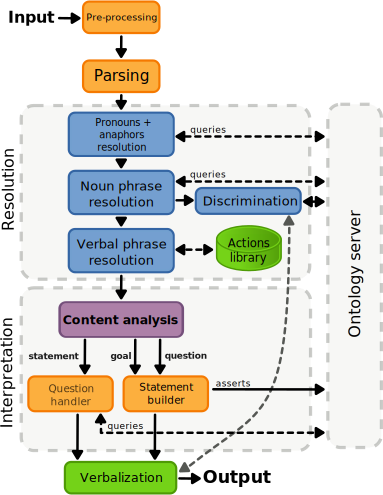
\includegraphics[width=0.6\linewidth]{images/dialogs/dialog_module_simple.pdf}
  \caption{The {\sc Dialogs} module has three main steps: the parsing,
  the interpretation and the verbalization. The interpretation module is
  responsible for both the \emph{resolution} and the semantic content
  \emph{analysis and translation}.} 
  \label{fig|dialog}
\end{figure}

As shown in Figure~\ref{fig|dialog}, the {\sc Dialogs} module is composed of
three main blocks. The user's input is first pre-processed. For instance,
\emph{I'm} constructs are expanded into \emph{I am} and then parsed. The parser
is a custom-made, rule-based (\ie grammar-free) tool that extracts the
grammatical structure from the user's sentence.

The result of the parsing is then sent to the \emph{interpretation} module, the
core of the approach.  Interpretation consists in three distinct operations:
the sentence \emph{resolution} (concepts grounding), the \emph{content
analysis} (what is the intent of the utterance: information, question or
desire) and the \emph{statement building} (translation into RDF statements).

The sentence resolution has three steps: {\it(1)} pronouns and anaphora are
replaced by, respectively, the correct speaker ID and the ID of the last object
spoken about (extracted from the dialogue history), {\it(2)} nominal groups are
disambiguated and grounded (noun phrase resolution), and {\it(3)} verbal groups
are resolved as well, and their associated thematic roles are retrieved (verbal
phrase resolution). Algorithm~\ref{algo|Resolution} describes the overall
process.  Next section describes specific examples to show how the noun and
verbal phrase resolution takes place.

\small
\begin{pseudocode}[ruled]{Resolution}{sentence, currentSpeaker}
\label{algo|Resolution}

\mathcal{G} \GETS \CALL{ParseNominalGroups}{sentence} \\

\FOREACH g \in \mathcal{G} \DO 
\BEGIN
   \mathcal{D} \GETS \CALL{GenerateDescription}{g} \STMTNUM{5.1em}{res.desc}\\
   candidates \GETS \CALL{Ontology.Find}{\mathcal{D}} \STMTNUM{4em}{res.onto}\\
   
   \IF \left|{candidates}\right| = 0 \THEN
    \BEGIN
      \OUTPUT{\mbox{Couldn't resolve the group!}} \\
      \EXIT \\
    \END
   \ELSEIF \left|{candidates}\right| = 1 \THEN
      id \GETS candidates[0] \STMTNUM{8em}{res.easy}\\

   \ELSE
      \BEGIN
	\IF \CALL{Ontology.CheckEquivalent}{candidates} \THEN
	  id \GETS candidates[0] \\
	\ELSE
	  id \GETS \CALL{Discrimination}{candidates} \\ %\STMTNUM{1em}{st.discrimination}\\
      \END \\
   \CALL{Replace}{g, id, sentence}
\END
\end{pseudocode}
\normalsize

As represented on Figure~\ref{fig|dialog}, interpretation tightly relies on the
communication with the knowledge base. All the concepts the robot manipulates
are stored in the \textit{ontology server} and retrieved through logical
queries, except for the verbs that are currently stored in a dedicated library
(the \emph{action library} on the diagram).

%%%%%%%%%%%%%%%%%%%%%%%%%%%%%%%%%%%%%
\section{Technical analysis}
\label{examples}

In order to better understand the overall process we next describe the
different steps based on three examples.

In this example, we assume some initial facts are present in the knowledge
base, both in the robot's \emph{own} model and in the \emph{human's} model.
Since the robot tries to ground a human utterance, all queries are sent 
to the \emph{human} model, \ie from the human perspective. 

\subsection{Informational content extraction}

Figure~\ref{dialog|ex1} shows a first example of human discourse grounding and
the extraction of informational content. We suppose that the robot knowledge
base only contains two initial statements in the human model. The user
asserts a new one: ``The yellow banana is big!''. 

\begin{figure}
    \centering
	\begin{tabular}{p{7cm}}
	\emph{Initial knowledge model of} \texttt{human\_01}\\
	\hline
    	\hspace{0.3cm}\stmt{banana\_01 \textbf{type} Banana} \\
    	\hspace{0.3cm}\stmt{banana\_01 \textbf{hasColor} yellow}\\
	
	\vspace{0.5em}
	\emph{Human input}\\
	\hline
	\hspace{0.3cm}``The yellow banana is big!'' \\

	\vspace{0.5em}
	\emph{Generated partial statements}\\
	\hline
	\hspace{0.3cm}\stmt{?obj \textbf{type} Banana} \\
    	\hspace{0.3cm}\stmt{?obj \textbf{hasColor} yellow} \\
    	\hspace{0.7cm}$\Rightarrow$ \stmt{?obj = banana\_01}\\

	\vspace{0.5em}
	\emph{Newly created statements}\\
	\hline
	\hspace{0.3cm}\stmt{banana\_01 \textbf{hasSize} big} \\
	\end{tabular}
\caption{First example of natural language grounding: the nominal group ``the
yellow banana'' is matched with the individual {\tt banana\_01}}.
\label{dialog|ex1}
\end{figure}


\small
\begin{pseudocode}[ruled]{GenerateDescription}{group}
\label{algo|GenerateDescription}

\PROCEDURE{GenerateDescription}{group} 
   noun \GETS \CALL{GetNoun}{group} \\ 
   \IF \CALL{Ontology.Lookup}{noun} \in (Instances) \STMTNUM{7.5em}{st.lookup} \THEN
   		\BEGIN
		id \GETS \CALL{Ontology.lookup}{noun}\\	
		\RETURN {\mathcal{D} + \{ *\ {\tt sameAs}\ <id> \}}\\
		\END
   \ELSE
    	\mathcal{D} = \mathcal{D} + \{ *\ {\tt type}\ <noun>\} \\
   
   \\
   det \GETS \CALL{GetDeterminant}{group} \\
   \IF det \in {\mbox(possessives)} \THEN
       \mathcal{D} = \mathcal{D} + \{ *\ {\tt isRelatedTo}\ <possessor>\} \\
    
    \IF det \in {\mbox(demonstratives)} \THEN
        \BEGIN
        \IF \CALL{Ontology.Check}{\{<currentSpeaker>\ {\tt focusesOn}\ *\}} \THEN 
            \mathcal{D} = \mathcal{D} + \{<currentSpeaker>\ {\tt focusesOn}\ *\}
        \ELSE
            \mathcal{D} = \mathcal{D} + \CALL{AnaphoricMatching}{} \STMTNUM{4em}{st.anaphoric} \\
        \END \\
   \\
   adjs \GETS \CALL{GetAdjectives}{group} \\
   \FOREACH adj \in adjs \DO
   	\BEGIN
   		\IF adj == <other> \THEN 
   			\BEGIN
   			id \GETS \CALL{History.GetMatchingGroup}{group} \STMTNUM{8em}{st.history}\\
   			\mathcal{D} = \mathcal{D} + \{ *\ {\tt differentFrom}\ <id> \}\\
   			\RETURN{D}\\
			\END   		
   		\ELSE
	     	\mathcal{D} = \mathcal{D} + \{ *\ {\tt hasFeature}\ <adj>\} \STMTNUM{9em}{st.adj} \\
    \END\\
    
   \\  
   nounComplements \GETS \CALL{GetNounComplements}{group} \\
   \FOREACH nouncmpl \in nounComplements \DO
     \mathcal{D} = \mathcal{D} + {\CALL{GenerateDescription}{nouncmpl}}\\
   
   
   \\  
   relativeClauses \GETS \CALL{GetSubordinateRelativeClauses}{group} \\
   \FOREACH relative \in relativeClauses \DO
   	\BEGIN
   	 \mathcal{G} \GETS \CALL{GetNominalGroups}{relative} \\
   	 \FOREACH g \in \mathcal{G} \DO
     	\mathcal{D} = \mathcal{D} + {\CALL{GenerateDescription}{g}}
    \END\\
     
   \\
   \RETURN{\mathcal{D}} 
\ENDPROCEDURE
\end{pseudocode}
\normalsize

\small
\begin{pseudocode}[ruled]{History.GetMatchingGroup}{group}
\label{algo|History}
\PROCEDURE{History.GetMatchingGroup}{group}
\COMMENT{Extract Nominal group from sentences stored in the history}\\
\mathcal{H} \GETS \CALL{History.GetAllNominalGoup}{}\\
\COMMENT{Generate description of the nominal group that is being processed.} \\
\COMMENT{The adjective  "other" is to be removed before calling this routine} \\
	\mathcal{G} \GETS \CALL{GenerateDescription}{group} \\ 
	
	candidates \GETS \mathcal{H} \cap \mathcal{G}\\
	\IF \left|{candidates}\right| = 0 \THEN
    \BEGIN
      \OUTPUT{\mbox{Couldn't find another object with the same characteristics!}} \\
      \EXIT \\
    \END
   \ELSEIF \left|{candidates}\right| = 1 \THEN
      id \GETS candidates[0]
   \ELSE
   	  id \GETS \CALL{Discrimination}{candidates}\\
   \RETURN{id}
\ENDPROCEDURE
\end{pseudocode}
\normalsize

We need to resolve the nominal group \emph{The yellow banana} to a known
concept.  A set of partial statements that describe the
concept is generated based on the grammatical parsing of the sentence
(algorithm~\ref{algo|GenerateDescription}). In the example, a banana
(\stmt{?obj \textbf{type} Banana}) that is yellow (\stmt{?obj \textbf{hasColor}
yellow})\footnote{Predicates like \concept{hasColor} or \concept{hasSize} that
bind \concept{banana\_01} to adjectives are extracted from a predefined
database of $[Predicate \rightarrow AdjectiveCategory]$, and falls back on the
generic \concept{hasFeature} predicate if the adjective is not known.}.  Based
on these partial statements a query is sent to the ontology server to retrieve
possible instances that match the description (algorithm~\ref{algo|Resolution},
\emph{(\ref{res.onto})}).

In this first simple case, the concept \concept{banana\_01} is unambiguously
matched (since there is only one possible banana) and returned. We can then add
the new information provided by the human, \ie the new statement
\stmt{banana\_01 \textbf{hasSize} big}, to the human model in the ontology
server.

\subsection{Intentional content through verb resolution}
The sentence in the first example is built with the state verb \emph{be} at
indicative. Let us examine a different example with an action verb at
imperative mode (\ie an order): ``Give me the banana". The process is
described in Figure~\ref{dialog|ex2}.

\begin{figure}
    \centering
	\begin{tabular}{p{7cm}}
	\emph{Initial knowledge model of} \texttt{human\_01}\\
	\hline
    	\hspace{0.3cm}\stmt{banana\_01 \textbf{type} Banana} \\
    	\hspace{0.3cm}\stmt{banana\_01 \textbf{hasColor} yellow}\\
	\end{tabular} \\

	\vspace{0.5em}

	\begin{tabular}{p{7cm}}
	\emph{Human input}\\
	\hline
    	\hspace{0.3cm}``Give me the banana.'' \\
	\end{tabular} \\

	\vspace{0.5em}

	\begin{tabular}{p{7cm}}
	\emph{Generated partial statements}\\
	\hline
    	\hspace{0.3cm}\stmt{?obj \textbf{type} Banana} \\
	\hspace{0.7cm}$\Rightarrow$ \stmt{?obj = banana\_01}\\

	\end{tabular} \\

	\vspace{0.5em}

	\begin{tabular}{p{7cm}}
	\emph{Newly created statements}\\
	\hline
    	\hspace{0.3cm}\stmt{human\_01 \textbf{desires} situation\_a3f74} \\
    	\hspace{0.3cm}\stmt{situation\_a3f74 \textbf{type} Give} \\
    	\hspace{0.3cm}\stmt{situation\_a3f74 \textbf{performedBy} myself} \\
    	\hspace{0.3cm}\stmt{situation\_a3f74 \textbf{actsOnObject} banana\_02} \\
    	\hspace{0.3cm}\stmt{situation\_a3f74 \textbf{receivedBy} human\_01} \\
	\end{tabular}

\caption{Second example: processing an order.}
\label{dialog|ex2}
\end{figure}

\label{processing_of_actions}

In order to capture the intentional content of a sentence (for example, an
order) we need to retain the semantics of the verb and its complements.
\emph{Thematic roles} allow to semantically link a verb to its complements.  We
use a small set of them that matches the relations the robot can actually
achieve. In this second example, the verb \emph{give} has three thematic roles:
\concept{performedBy}, \concept{actsOnObject} and \concept{receivedBy}.

The list of actions the robot can plan for (currently \emph{take},
\emph{place}, \emph{give}, \emph{show}, \emph{hide} and \emph{move}) along with
possible synonyms and their associated thematic roles are stored in a
predefined library of actions (Figure~\ref{fig|dialog}). For each action we identify and store the role
of the subject of the sentence --- always \concept{performedBy}; the role of
the direct object (for instance, \concept{actsOnObject}); and the role of each
of the indirect objects with their optional prepositions (for instance,
\concept{receivedBy})\footnote{Note that in example 2, ``give me the banana'',
the pronoun ``me'' appears before ``banana'', while it is an indirect
complement --- ``give it {\bf to me}''. The parser correctly handles these
cases.}. Moreover, we check with the help of the ontology that each holder of a
role has a consistent semantic. For instance, action \emph{Give} must have a
manipulable physical item (\emph{Artifact}) as direct object. Thus, if the
concept the robot finds for the thematic role \emph{actsOnObject} can not be
inferred to be an artifact, it goes back to the human saying it does not
understand.

Once the sentence is completely resolved and translated into a formal
representation (a human desire in this case\footnote{Orders are here
represented as human desires: the human desires a specific new situation.}), we
store it in the ontology server. The robot's decisional/executive layers should
then decide whether to execute the order or not. 

\subsection{Informational content extraction requiring clarification}
\begin{figure}
    \centering
	\begin{tabular}{p{7cm}}
	\emph{Initial knowledge model of} \texttt{human\_01}\\
	\hline
     	\hspace{0.3cm}\stmt{banana\_01 \textbf{type} Banana} \\
     	\hspace{0.3cm}\stmt{banana\_01 \textbf{hasColor} yellow} \\
     	\hspace{0.3cm}\stmt{banana\_02 \textbf{type} Banana} \\
     	\hspace{0.3cm}\stmt{banana\_02 \textbf{hasColor} green} \\
	\end{tabular} \\

	\vspace{0.5em}

	\begin{tabular}{p{7cm}}
	\emph{Human input}\\
	\hline
     	\hspace{0.3cm}``The banana is good.'' \\
	\end{tabular} \\

	\vspace{0.5em}

	\begin{tabular}{p{7cm}}
	\emph{Generated partial statements}\\
	\hline
     	\hspace{0.3cm}\stmt{?obj \textbf{type} Banana} \\
	\end{tabular} \\

	\vspace{0.5em}

	\begin{tabular}{p{7cm}}
	\emph{Robot output speech}\\
	\hline
     	\hspace{0.3cm}``The yellow one or the green one?'' \\
	\end{tabular} \\

	\vspace{0.5em}

	\begin{tabular}{p{7cm}}
	\emph{Human answer}\\
	\hline
     	\hspace{0.3cm}``The green one.'' \\
	\end{tabular} \\
    
	\vspace{0.5em}

	\begin{tabular}{p{7cm}}
	\emph{Newly created statements}\\
	\hline
     	\hspace{0.3cm}\stmt{banana\_02 \textbf{hasFeature} good} \\
	\end{tabular}

\caption{Ambiguity resolution: in this example, ``banana'' can refer to the
yellow banana (\concept{banana\_01}) or the green one (\concept{banana\_02}).
Discrimination routines handle the disambiguation process.} \label{dialog|ex3}
\end{figure}

This last example (Figure~\ref{dialog|ex3}) shows the resolution of ambiguous
concepts. In this case the user refers to ``the banana'' while two instances of
the \concept{Banana} class exist in the ontology. The robot needs to find out
to which instance the user is actually referring to. To this end,
disambiguation routines~\cite{Ros2010b} find differences between the instances
(in the example, one banana is yellow while the other one is green) and build a
sentence through the \emph{verbalization} module to ask the user a closed
question that will help clarify the ambiguity: ``Is it yellow or green?'' The
user's answer is parsed and added to the previous sentence. The resulting,
augmented, sentence (\ie ``Give me the green banana") goes again through all
the interpretation steps. This process is repeated until no ambiguities arise.
In the example, the \concept{banana\_02} is finally returned.

Several other strategies are used in parallel to disambiguate concepts without
having to ask for more information to the human: 

\begin{itemize}
	\item Which objects are currently visible to the human? If only one of
	them, then it is probably the one the user is talking about. 
	\item Did a previous interaction involved a specific object that would
	still be the subject of the current sentence?
	\item Is the user looking or pointing to a specific object?
\end{itemize}
 
While no examples involving questions have been detailled, \emph{W-} questions
and \emph{yes/no} questions can be processed in a similar way by
\textsc{Dialogs}. For instance, a question like: \emph{What is on the table?}
is grounded (to extract the relation \emph{isOn} and to find what \emph{table}
refers to) and transformed into the following kind of query: {\tt find ?var [?var isOn
table1]}.  Answers are converted back to a full sentence and uttered to the
human.


The next chapter (page~\pageref{chapter|evaluation}) presents several
experiments that make intensive use of the {\tt Dialogs} module.

\section{Planing for interaction}
\label{sect|planing-for-interaction}

\fxerror{TDB: dialogue + planing should allow the robot to answer questions
requiring temporal projection like: "Can you go to this place?"}


\chapter{Evaluation}
\label{chapter|evaluation}

\section{Comparison of oro-server with other existing systems}
\label{sect|evaluation-oroserver}

\section{Experimental evaluation}
\label{sect|experimental-evaluation}

\subsection{Experimental setup}
\label{sect|user-experiments}

\subsection{Simulation of HRI interaction}
\label{sect|simulation}


\subsection{User studies}
\label{sect|userstudies}



\chapter{Conclusion}
\label{chapter|conclusion}

\section{Scientific contributions}
\label{sect|scientific-contributions}

\section{Technical contributions}
\label{sect|technical-contributions}


\printglossaries

\bibliographystyle{ieeetr}
\bibliography{/home/slemaign/work/biblio/biblio_phd_severin}


%%%%%%%%%%%%%%%%%%%%%%%%%%%%%%%%%%%%%%%%%%%%%%%%%%%%%%%%%%%%%%%%%%%%%%%%%%%%%%%%%%%%%%%%%%%%%%%%%%%%%%%

\end{document}


